\documentclass[11pt]{article}
\usepackage{geometry}                
\geometry{letterpaper}                   

\usepackage{graphicx}
\usepackage{amssymb}
\usepackage{epstopdf}
\usepackage[numbers]{natbib}
\usepackage{amssymb, amsmath ,empheq}
\DeclareGraphicsRule{.tif}{png}{.png}{`convert #1 `dirname #1`/`basename #1 .tif`.png}

%\title{Title}
%\author{Name 1, Name 2}
%\date{date} 

\begin{document}



\thispagestyle{empty}

\begin{center}
\includegraphics[width=5cm]{ETHlogo.eps}

\bigskip


\bigskip


\bigskip


\LARGE{ 	Lecture with Computer Exercises:\\ }
\LARGE{ Modelling and Simulating Social Systems with MATLAB\\}

\bigskip

\bigskip

\small{Project Report}\\

\bigskip

\bigskip

\bigskip

\bigskip


\begin{tabular}{|c|}
\hline
\\
\textbf{\LARGE{Simulation of the Information Spreading}}\\
\textbf{\LARGE{in a Facebook Network}}\\
\\
\hline
\end{tabular}
\bigskip

\bigskip

\bigskip

\LARGE{Name 1 \& Name 2}



\bigskip

\bigskip

\bigskip

\bigskip

\bigskip

\bigskip

\bigskip

\bigskip

Zurich\\
December 2013\\

\end{center}



\newpage

%%%%%%%%%%%%%%%%%%%%%%%%%%%%%%%%%%%%%%%%%%%%%%%%%

\newpage
\section*{Agreement for free-download}
\bigskip


\bigskip


\large We hereby agree to make our source code for this project freely available for download from the web pages of the SOMS chair. Furthermore, we assure that all source code is written by ourselves and is not violating any copyright restrictions.

\begin{center}

\bigskip


\bigskip


\begin{tabular}{@{}p{4cm}@{}p{4cm}@{}@{}p{4cm}@{}}

\begin{minipage}{4cm}
\vspace{2cm}
\large Urs Lustenberger
\end{minipage}

&

\begin{minipage}{4cm}

\vspace{2cm}
 \large \hspace{4mm} Nino Wili

\end{minipage}

&

\begin{minipage}{4cm}
\vspace{2cm}
\large Patric Z\"ochbauer

\end{minipage}
\end{tabular}


\end{center}
\newpage

%%%%%%%%%%%%%%%%%%%%%%%%%%%%%%%%%%%%%%%



% IMPORTANT
% you MUST include the ETH declaration of originality here; it is available for download on the course website or at http://www.ethz.ch/faculty/exams/plagiarism/index_EN; it can be printed as pdf and should be filled out in handwriting


%%%%%%%%%% Table of content %%%%%%%%%%%%%%%%%

\tableofcontents

\newpage

%%%%%%%%%%%%%%%%%%%%%%%%%%%%%%%%%%%%%%%



\section{Abstract}

\section{Individual contributions}

\section{Introduction and Motivations}

\subsection{Introduction and fundamental questions}

Social Networks like facebook and twitter are growing very fast. Most young people like students do have an account in one ore more of them. Many articles, pictures and videos on the internet have a direct "share" button. It is a very interesting question how information spreads in such networks. First, the internet may have become the fastest and sometimes most important source of "news" and information beside the "traditional" media and second, companies seem to be very interested in "informing" the right people with their commercials. 
\\
\\
The simplest way to describe the information spreading uses similarities to epidemiology, which means that the flow of information of one person to another is looked at as an "infection". In this work, we implemented a simple model in a homogeneous way with a set of differential equations and their numeric solutions as well as an agent-based, heterogeneous model, using a real facebook network.
\\
The fundamental questions of this work are:

\begin{itemize}
\item Are there relevant differences in the time evolution of the homogeneous and the agent-based network?

\item Are there indiviuals which are more important to the spreading of information (also called influentials)? Can they be recognized in the sense of position and connectivity in the network?
\end{itemize}

\subsection{Motivation}

As the team of authors consists of two chemists and a mathematician, the personal motivations also have a broad range. We were glad to recognize the parallels between our simulations with statistical physics and chemical reaction kinetics... 
















\section{Description of the Model}

The process of information spreading has many similarities with epidemiology, therefore the well known SIR-model was adapted\cite{complexsystems}.  The ``susceptibles'', are not aware of the information and are called ``ignorants'' within this work. ``Infected'' individuals know about the information and are willing to share it with other people, in other words they spread it and are therefore called ``spreaders''. The adaptation of the epidemiological term ``recovered'' is not that straightforward as its meaning in this context is not entirely clear. However, they can be interpreted as individuals being aware of the information but do not share it with others. They are called "stiflers".
\\
\\
In the SIR-model as well as in the agent-based model, the following set of ``reaction equations'' was used (I: Ignorant, S: Spreader, R: Stifler):


\begin{empheq}[left=\empheqlbrace]{align}
& I + S \xrightarrow{\lambda} 2 S \\
& S + R \xrightarrow{\alpha} 2 R \\
& S + S \xrightarrow{\alpha} S + R 
\end{empheq}
\newline
The main difference to the standard SIR-model is that spreaders do not become stiflers spontaneously. This change is only induced by meeting another spreader or stifler.

\subsection{Homogeneous SIR model}

In the mathematical treatment of the homogeneous model, the set of differential equations is expressed in terms of the densities $i(t)=I(t)/N$, $s(t)=S(t)/N$ and $r(t)=R(t)/N$, where N is the number of individuals in the network.

\begin{empheq}[left=\empheqlbrace]{align}
& \frac{\text{d}i(t)}{\text{d}t} = -\lambda \cdot s(t)i(t) \\
& \frac{\text{d}s(t)}{\text{d}t} = \lambda \cdot s(t)i(t) - \alpha \cdot s(t)[s(t)+r(t)] \\
& \frac{\text{d}r(t)}{\text{d}t} = \alpha \cdot s(t)[s(t)+r(t)]
\end{empheq}



\subsection{Agent-based model}

In the inhomogeneous, agent-based model the individuals are connected in a certain manner (facebook friends in this particular work). Only connected agents are able to meet. If a meeting occurs, transitions are induced at a certain probability depending on the relation between the agents (details are discussed later). Additional to the different connectivity of the agents, they also have a different activity, i.e. different probability to meet somebody. 
\\
\\
To convert the reaction equations into an agent-based model, time was discretized and in each time step a series of two steps is performed. First, the agents randomly meet another agent they know or nobody. Only two-agent meetings are possible. In the second step, the status of the agents change corresponding to the situation. There are six possible combinations of ignorants, spreaders and stiflers. Three of them correspond to the ``reactions'' 1-3, the other ones (I+I, I+R and R+R) have no other influence than ``occupying'' the agents. The probability $\lambda$ was chosen to be dependent on the number of common friends. For simplicity, $\alpha$ was a constant.


\section{Implementation}

\subsection{The Network}
how did we get the network?

how did we get the coordinates with gephi?

how was the code implemented? (how detailed does this have to be? references to matlab files?)

\section{Simulation Results and Discussion}

most important question!

\section{Summary and Outlook}

%%%%%%%%%%%

\begin{thebibliography}{9}

\bibitem{complexsystems}{
	A. Barrat, M. Barthélemy, A. Vespignani.
\newblock Dynamical Processes on Complex Networks.
\newblock \textit{Cambridge University Press}
\newblock Chapter 10, pp. 216-241

}

\bibitem{influentials}{
	D.J.Watts, P.S.Dodds.
\newblock Influentials, Networks, and Public Opinion Formation.
\newblock \textit{Journal of Consumer Research}
\newblock Vol 34, No. 4 (December 2007), pp. 441-458
}
	


\end{thebibliography}

\section{Additional figures}

\begin{figure}
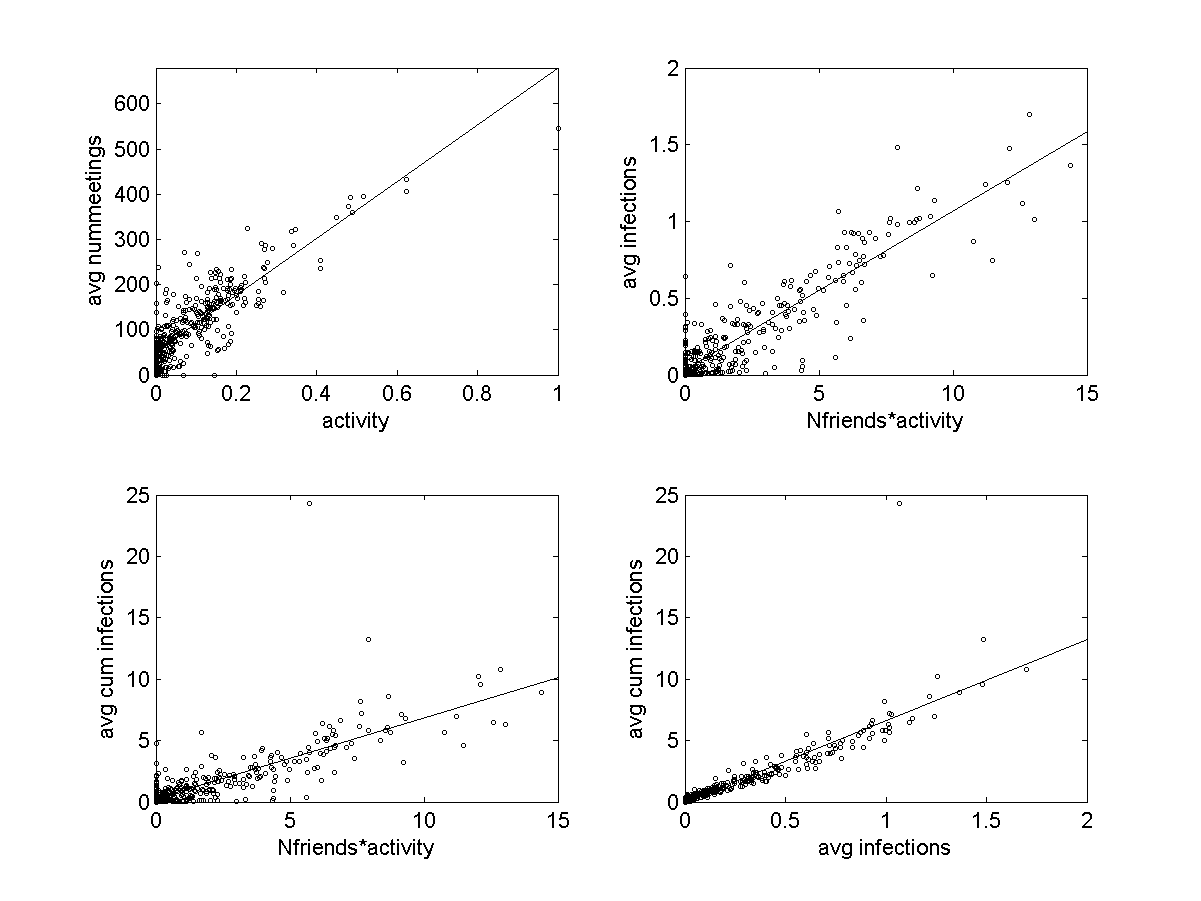
\includegraphics[width=7cm]{ImportantCorrelations}
\caption{sdlhfa}
\label{ImportantCorrelations}
\end{figure}

\begin{figure}
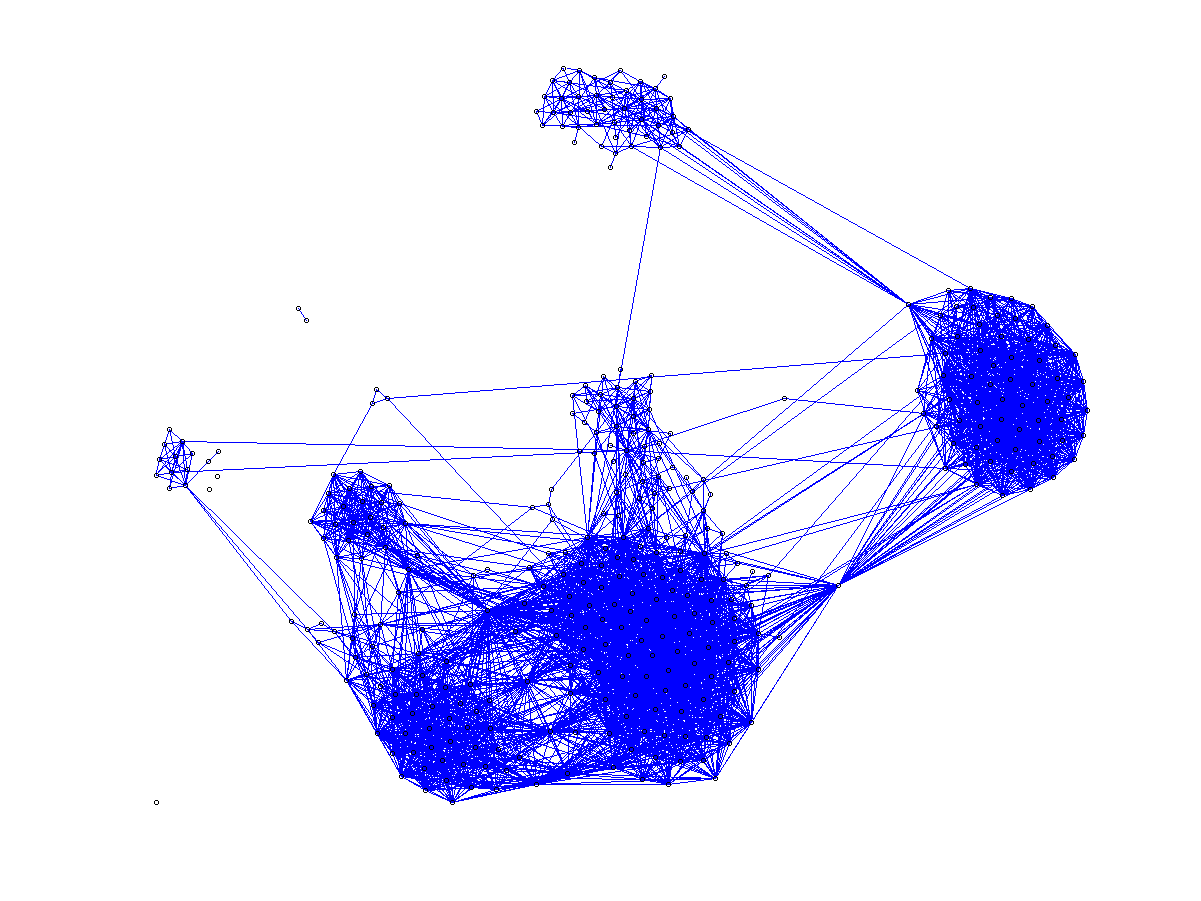
\includegraphics[width=7cm]{Network-Graph}
\caption{sdlhfa}
\label{Network-Graph}
\end{figure}





\end{document}  



 
